%%
%% This is file `template-8s.tex',
%% generated with the docstrip utility.
%%
%% The original source files were:
%%
%% template.raw  (with options: `8s')
%% 
%% Template for the LaTeX class aipproc.
%% 
%% (C) 1998,2000,2001 American Institute of Physics and Frank Mittelbach
%% All rights reserved
%% 
%%
%% $Id: template.raw,v 1.12 2005/07/06 19:22:14 frank Exp $
%%

%%%%%%%%%%%%%%%%%%%%%%%%%%%%%%%%%%%%%%%%%%%%
%% Please remove the next line of code if you
%% are satisfied that your installation is
%% complete and working.
%%
%% It is only there to help you in detecting
%% potential problems.
%%%%%%%%%%%%%%%%%%%%%%%%%%%%%%%%%%%%%%%%%%%%

%
% $Id: aipcheck.tex,v 1.9 2005/12/01 16:16:27 frank Exp $
%
%%%%%%%%%%%%%%%%%%%%%%%%%%%%%%%%%%%%%%%%%%%%%%%%%%
% Testing for potential problems with this class
%%%%%%%%%%%%%%%%%%%%%%%%%%%%%%%%%%%%%%%%%%%%%%%%%%

\newif\ifproblem
\newif\ifobservation
\newif\iftimesok

\makeatletter
\def\IfStandaloneCheck{\def\next{aipcheck}
  \edef\currjob{\jobname}
  \edef\next{\meaning\next}
  \edef\currjob{\meaning\currjob}
  \ifx\currjob\next
    \expandafter\@firstoftwo
  \else
    \expandafter\@secondoftwo
  \fi
}
\makeatother

\typeout{***********************************************}
\typeout{*}
\typeout{* Testing if all files required for the aipproc}
\typeout{* class are available ...}
\typeout{*}
\typeout{***********************************************}

\typeout{*}
\typeout{* Looking for LaTeX2e ... }
\ifx\documentclass\undefined
 \typeout{*}
 \typeout{* Sorry this is a fatal error:}
 \typeout{*}
 \typeout{* The aipproc class can only be used with LaTeX2e which is}
 \typeout{* the standard LaTeX since 1994!}
 \typeout{*}
 \typeout{* Please make sure that your version of LaTeX is up-to-date}
 \typeout{* before attempting to use this class.}
 \typeout{*}
 \expandafter\stop
\else
 \typeout{* ... ok }
\fi


\def\next#1/#2/#3\next{#1#2}
\typeout{*}
\typeout{* Testing that LaTeX2e is not too old ... }
\ifnum\expandafter\next\fmtversion\next<199612 \relax
 \typeout{* ... what a vintage! }
 \typeout{*}
 \typeout{* Sorry this is a fatal error:}
 \typeout{*}
 \typeout{* The aipproc class can only be used with a recent version}
 \typeout{* of LaTeX2e. Your version is dated \fmtversion\space --- but}
 \typeout{* at least the 1996/12/01 version is required!}
 \typeout{*}
 \typeout{* Please make sure that your version of LaTeX is up-to-date}
 \typeout{* before attempting to use this class.}
 \typeout{*}
 \expandafter\stop
\else
 \ifnum\expandafter\next\fmtversion\next<199806 \relax
   \typeout{* ... probably ok }
   \typeout{*}
   \typeout{* Your version of LaTeX2e is quite old --- the aipproc class}
   \typeout{* hasn't been tested with your release.}
   \typeout{*}
   \typeout{* We believe that it will probably work, but if you encounter}
   \typeout{* problems you will need upgrade your installation.}
   \typeout{*}
   \typein{* Type <return> to continue ...}
   \problemtrue
 \else
   \typeout{* ... ok }
 \fi
\fi


\typeout{*}
\typeout{* Looking for aipproc.cls ... }
\IfFileExists{aipproc.cls}
    {
     \typeout{* ... ok }
    }
    {
     \typeout{* ... not found! }
     \typeout{*}
     \typeout{* Sorry this is a fatal error:}
     \typeout{*}
     \typeout{* Before you can use the aipproc class you have to unpack}
     \typeout{* it from the documented source.}
     \typeout{*}
     \typeout{* Run LaTeX on the file 'aipproc.ins', e.g.,}
     \typeout{*}
     \typeout{* \space\space latex aipproc.ins}
     \typeout{*}
     \typeout{* or whatever is necessary on your installation to process}
     \typeout{* a file with LaTeX. This should unpack a number of files for you:}
     \typeout{*}
     \typeout{* aipproc.cls \space and \space aip-*.clo}
     \typeout{*}
     \typeout{* After that retry processing this guide.}
     \typeout{*}
     \stop
}

\typeout{*}
\typeout{* Looking for aipxfm.sty ... }
\IfFileExists{aipxfm.sty}
    {
     \typeout{* ... ok }
    }
    {
     \typeout{* ... not found! }
     \typeout{*}
     \typeout{* Sorry this is a fatal error:}
     \typeout{*}
     \typeout{* The aipxfm.sty file which is part of the aipproc distribution}
     \typeout{* must be installed in a directory which is searched by LaTeX.}
     \typeout{*}
     \typeout{* Please install this file and retry.}
     \typeout{*}
     \stop
}

\typeout{*}
\typeout{* Looking for aip-8s.clo ... }
\IfFileExists{aip-8s.clo}
    {
     \typeout{* ... ok }
    }
    {
     \typeout{* ... not found! }
     \typeout{*}
     \typeout{* Sorry this is a fatal error:}
     \typeout{*}
     \typeout{* The aip-8s.clo file which is part of the aipproc distribution}
     \typeout{* must be installed in a directory which is searched by LaTeX.}
     \typeout{*}
     \typeout{* Please install this file and retry.}
     \typeout{*}
     \stop
}

\typeout{*}
\typeout{* Looking for aip-8d.clo ... }
\IfFileExists{aip-8d.clo}
    {
     \typeout{* ... ok }
    }
    {
     \typeout{* ... not found! }
     \typeout{*}
     \typeout{* Sorry this is a fatal error:}
     \typeout{*}
     \typeout{* The aip-8d.clo file which is part of the aipproc distribution}
     \typeout{* must be installed in a directory which is searched by LaTeX.}
     \typeout{*}
     \typeout{* Please install this file and retry.}
     \typeout{*}
     \stop
}


\typeout{*}
\typeout{* Looking for aip-6s.clo ... }
\IfFileExists{aip-6s.clo}
    {
     \typeout{* ... ok }
    }
    {
     \typeout{* ... not found! }
     \typeout{*}
     \typeout{* Sorry this is a fatal error:}
     \typeout{*}
     \typeout{* The aip-6s.clo file which is part of the aipproc distribution}
     \typeout{* must be installed in a directory which is searched by LaTeX.}
     \typeout{*}
     \typeout{* Please install this file and retry.}
     \typeout{*}
     \stop
}


\iffalse
\typeout{*}
\typeout{* Looking for aip-arlo.clo ... }
\IfFileExists{aip-arlo.clo}
    {
     \typeout{* ... ok }
    }
    {
     \typeout{* ... not found! }
     \typeout{*}
     \typeout{* Sorry this is a fatal error:}
     \typeout{*}
     \typeout{* The aip-arlo.clo file which is part of the aipproc distribution}
     \typeout{* must be installed in a directory which is searched by LaTeX.}
     \typeout{*}
     \typeout{* Please install this file and retry.}
     \typeout{*}
     \stop
}
\fi

\typeout{*}
\typeout{* Looking for fixltx2e.sty ... }
\IfFileExists{fixltx2e.sty}
    {
     \typeout{* ... ok }
    }
    {
     \typeout{* ... not found, trying fix2col.sty instead ... }
     \typeout{*}
     \IfFileExists{fix2col.sty}
         {
          \typeout{* ... ok }
         }
         {
          \typeout{* ... not found! }
          \typeout{*}
          \typeout{* Sorry this is a fatal error:}
          \typeout{*}
          \typeout{* Your LaTeX distribution contains neither fixltx2e.sty}
          \typeout{* nor fix2col.sty.}
          \typeout{*}
          \typeout{* This means that it is either too old or incompletely}
          \typeout{* installed.}
          \typeout{*}
          \typeout{* fixltx2e.sty is part of the standard LaTeX distribution}
          \typeout{* since 1999; fix2col.sty is an earlier version of this}
          \typeout{* package.}
          \typeout{*}
          \typeout{* Best solution is to get the latest LaTeX distribution.}
          \typeout{* If this is impossible for you, download fix2col.sty.}
          \typeout{* You can get this software from a CTAN host.}
          \typeout{* Refer to http://www.ctan.org and search for "fix2col".}
          \typeout{*}
          \typeout{* After you have updated your LaTeX distribution}
          \typeout{* retry processing this guide.}
          \stop
     }
}

\typeout{*}
\typeout{* Looking for fontenc.sty ... }
\IfFileExists{fontenc.sty}
    {
     \typeout{* ... ok }
    }
    {
     \typeout{* ... not found! }
     \typeout{*}
     \typeout{* Sorry this is a fatal error:}
     \typeout{*}
     \typeout{* The fontenc package, which is part of standard LaTeX}
     \typeout{* (base distribution) has to be installed at the site to}
     \typeout{* run the aipproc class.}
     \typeout{*}
     \typeout{* The fact that it cannot be found either means that}
     \typeout{* this LaTeX release is too old or that it was installed}
     \typeout{* improperly.}
     \typeout{*}
     \typeout{* Please make sure that your version of LaTeX is okay}
     \typeout{* before attempting to use this class. The LaTeX distribution}
     \typeout{* contains the file "ltxcheck.tex" which can be used to}
     \typeout{* test the basic functionality and integrity of your installation.}
     \typeout{*}
     \stop
    }

\typeout{*}
\typeout{* Looking for calc.sty ... }
\IfFileExists{calc.sty}
    {
     \typeout{* ... ok }
    }
    {
     \typeout{* ... not found! }
     \typeout{*}
     \typeout{* Sorry this is a fatal error:}
     \typeout{*}
     \typeout{* The calc package, which is part of standard LaTeX}
     \typeout{* (tool distribution) has to be installed at the site}
     \typeout{* to run the aipproc class.}
     \typeout{*}
     \typeout{* The fact that it cannot be found either means that}
     \typeout{* this LaTeX release is too old or that it was installed}
     \typeout{* only in parts.}
     \typeout{*}
     \typeout{* Please make sure that the tools distribution of LaTeX}
     \typeout{* is installed before attempting to use this class.}
     \typeout{*}
     \typeout{* (You might be able to get calc.sty separately for your}
     \typeout{* installation if you are unable to upgrade to a recent}
     \typeout{* distribution for some reason.)}
     \typeout{*}
     \stop
    }

\typeout{*}
\typeout{* Looking for varioref.sty ... }
\IfFileExists{varioref.sty}
    {
     \typeout{* ... ok }
     \gdef\variorefoptionifavailable{varioref,}
    }
    {
     \typeout{* ... not found! }
     \typeout{*}
     \typeout{* Problem detected:}
     \typeout{*}
     \typeout{* The varioref package, which is part of standard LaTeX}
     \typeout{* (tool distribution) is not installed at this site.}
     \typeout{*}
     \typeout{* The fact that it cannot be found either means that}
     \typeout{* this LaTeX release is too old or that it was installed}
     \typeout{* only in parts.}
     \typeout{*}
     \typeout{* You can use the aipproc class without this package but }
     \typeout{* you cannot make use of the options "varioref" or "nonvarioref".}
     \typeout{*}
     \typeout{* Please also note that the aipguide.tex documentation}
     \typeout{* normally uses the "varioref" option to show its}
     \typeout{* effects (which  will now fail).}
     \typeout{*}
     \typein{* Type <return> to continue ...}
     \problemtrue
     \gdef\variorefoptionifavailable{}
     \let\vpageref\pageref
     \let\vref\ref
    }

\typeout{*}
\typeout{* Looking for times.sty ... }
\IfFileExists{times.sty}
    {
     \begingroup
% load times and forget it immediately again
       \RequirePackage{times}
       \global\expandafter\let\csname ver@times.sty\endcsname\relax    
       \long\def\next{ptm}
       \ifx\rmdefault\next
         \typeout{* ... ok }
         \gdef\psnfssproblemoption{}
         \endgroup
         \timesoktrue
       \else
         \endgroup
     \typeout{* ... obsolete! }
     \typeout{*}
     \typeout{* Serious problem detected:}
     \typeout{*}
     \typeout{* The times package, which is part of standard LaTeX}
     \typeout{* (psnfss distribution) is obsolete at this site.}
     \typeout{*}
     \typeout{* The fact that it contains incorrect code either means that}
     \typeout{* this LaTeX release is too old or that it was installed}
     \typeout{* only in parts with old files remaining!}
     \typeout{*}
     \typeout{* You can use the aipproc class without this package but}
     \typeout{* you have to specify the option "cmfonts" which result in}
     \typeout{* documents which are not conforming to the AIP layout specification!}
     \typeout{*}
     \typeout{* You can also try using the class in the following way:}
     \typeout{*}
     \typeout{* \space\space \string\documentclass[cmfonts]{aipproc}}
     \typeout{* \space\space \string\usepackage{times}}
     \typeout{* \space\space ...}
     \typeout{*}
     \typeout{* With luck this will result in Times Roman output but chances}
     \typeout{* are that you will get a larger number of error messages in}
     \typeout{* which case you have to remove the \string\usepackage declaration.}
     \typeout{*}
     \typein{* Type <return> to continue ...}
          \problemtrue
          \gdef\psnfssproblemoption{cmfonts}
          \def\textdegree{$^\circ$}            % used below but now
                                               % not setup
       \fi
    }
    {
     \typeout{* ... not found! }
     \typeout{*}
     \typeout{* Serious problem detected:}
     \typeout{*}
     \typeout{* The times package, which is part of standard LaTeX}
     \typeout{* (psnfss distribution) can not be found.}
     \typeout{*}
     \typeout{* The fact that this package cannot be found either means that}
     \typeout{* this LaTeX release is too old or that it was installed}
     \typeout{* only in parts!}
     \typeout{*}
     \typeout{* You can use the aipproc class without this package but }
     \typeout{* you have to specify the option "cmfonts" which result in}
     \typeout{* documents which are not conforming to the AIP layout specification!}
     \typeout{*}
     \typein{* Type <return> to continue ...}
     \problemtrue
     \gdef\psnfssproblemoption{cmfonts,}
    }

\iftimesok % don't bother testing other font options if times already
           % bad

\typeout{*}
\typeout{* Looking for t1ptm.fd or T1ptm.fd ... }
\IfFileExists{t1ptm.fd}
    {
     \typeout{* ... ok }
    }
    {
     \typeout{* ... not found, trying T1ptm.fd ... }
     \IfFileExists{T1ptm.fd}
          {
           \typeout{* ... ok }
          }
          {
           \typeout{* ... not found}
           \typeout{* Serious problem detected:}
           \typeout{*}
           \typeout{* The times package, which is part of standard LaTeX}
           \typeout{* (psnfss distribution) is available but the corresponding}
           \typeout{* .fd file (defining how to load Times Roman) is missing.}
           \typeout{*}
           \typeout{* The fact that this package is only partially installed}
           \typeout{* means that you LaTeX installation is unable to use Times}
           \typeout{* Roman fonts!}
           \typeout{*}
           \typeout{* You can use the aipproc class without this package but }
           \typeout{* you have to specify the option "cmfonts" which result in}
           \typeout{* documents which are not conforming to the AIP layout}
           \typeout{* specification!}
           \typeout{*}
           \typein{* Type <return> to continue ...}
           \problemtrue
           \timesokfalse
           \gdef\psnfssproblemoption{cmfonts,}
          }
    }

\fi


\newcommand\CheckFDFile[3]{%
  \typeout{*}
  \typeout{* Looking for #1#3.fd or #2#3.fd ... }
  \IfFileExists{#1#3.fd}
    {
     \typeout{* ... ok }
    }
    {
     \IfFileExists{#2#3.fd}
      {
       \typeout{* ... ok }
      }
      {\problemtrue
       \typeout{* ... not found! }
      }
    }
}

\iftimesok % don't bother testing other font options if Times already bad

%\CheckFDFile{ot1}{OT1}{ot1ztmcm}
%\CheckFDFile{oml}{OML}{omlztmcm}
%\CheckFDFile{oms}{OMS}{omsztmcm}
%\CheckFDFile{omx}{OMX}{omxztmcm}

\typeout{*}
\typeout{* Looking for mathptm.sty ... }
\IfFileExists{mathptm.sty}
    {
     \typeout{* ... ok }
     \CheckFDFile{ot1}{OT1}{ptmcm}
     \CheckFDFile{oml}{OML}{ptmcm}
     \CheckFDFile{oms}{OMS}{pzccm}
     \CheckFDFile{omx}{OMX}{psycm}
     \ifproblem
      \typeout{*}
      \typeout{* Problem detected:}
      \typeout{*}
      \typeout{* The mathptm package, which is part of standard LaTeX}
      \typeout{* (psnfss distribution) was found but some or all of its}
      \typeout{* support files describing which fonts to load are missing!}
      \typeout{*}
      \typeout{*}
      \typeout{* The fact that this package is only partially installed}
      \typeout{* means that the mathptm package cannot be used!}
      \typeout{*}
      \typeout{* You can use the aipproc class without this package but }
      \typeout{* you have to specify the option "nomathfonts" so that}
      \typeout{* math formulas will be typeset using Computer Modern.}
      \typeout{*}
      \typein{* Type <return> to continue ...}
      \problemtrue
      \gdef\psnfssproblemoption{nomathfonts,}
     \else
      \typeout{*}
      \typeout{* Looking for mathptmx.sty ... }
      \IfFileExists{mathptmx.sty}
       {
        \typeout{* ... ok }
        \CheckFDFile{ot1}{OT1}{ztmcm}
        \CheckFDFile{oml}{OML}{ztmcm}
        \CheckFDFile{oms}{OMS}{ztmcm}
        \CheckFDFile{omx}{OMX}{ztmcm}
        \ifproblem
          \typeout{*}
          \typeout{* Problem detected:}
          \typeout{*}
          \typeout{* The mathptmx package, which is part of standard LaTeX}
          \typeout{* (psnfss distribution) was found but some or all of its}
          \typeout{* support files describing which fonts to load are missing!}
          \typeout{*}
          \typeout{*}
          \typeout{* The fact that this package is only partially installed}
          \typeout{* means that the mathptmx package cannot be used!}
          \typeout{*}
          \typeout{* You can use the aipproc class without this package but }
          \typeout{* you have to specify the option "mathptm" (no x) so that}
          \typeout{* math formulas use the older version with upright greek letters.}
          \typeout{*}
          \typein{* Type <return> to continue ...}
          \problemtrue
          \gdef\psnfssproblemoption{mathptm,}
        \fi
       }
       {
        \typeout{* ... not found! }
        \typeout{*}
        \typeout{* Problem detected:}
        \typeout{*}
        \typeout{* The mathptmx package, which is part of standard LaTeX}
        \typeout{* (psnfss distribution) can not be found.}
        \typeout{*}
        \typeout{* This is unfortunate but not a disaster as the older}
        \typeout{* version of the package "mathptm" (no x) seems to exist.}
        \typeout{*}
        \typeout{* You can use the aipproc class without this package but }
        \typeout{* you have to specify the option "mathptm" so that}
        \typeout{* math formulas use the older version with upright greek letters.}
        \typeout{*}
        \typein{* Type <return> to continue ...}
        \problemtrue
        \gdef\psnfssproblemoption{mathptm,}
       }
      \fi
    }
    {
     \typeout{* ... not found! }
     \typeout{*}
     \typeout{* Problem detected:}
     \typeout{*}
     \typeout{* The mathptm package, which is part of standard LaTeX}
     \typeout{* (psnfss distribution) can not be found.}
     \typeout{*}
     \typeout{* The fact that this package cannot be found either means that}
     \typeout{* this LaTeX release is too old or that it was installed}
     \typeout{* only in parts!}
     \typeout{*}
     \typeout{* You can use the aipproc class without this package but }
     \typeout{* you have to specify the option "nomathfonts" so that}
     \typeout{* math formulas will be typeset using Computer Modern.}
     \typeout{*}
     \typein{* Type <return> to continue ...}
     \problemtrue
     \gdef\psnfssproblemoption{nomathfonts,}
    }

\typeout{*}
\typeout{* Looking for mathtime.sty ... }
\IfFileExists{mathtime.sty}
    {
     \typeout{* ... ok }
    }
    {
     \typeout{* ... not found! }
     \typeout{*}
     \typeout{* The mathime package can not be found.}
     \typeout{*}
     \typeout{* This is not a real problem but an observation,}
     \typeout{* because this package is only of interest}
     \typeout{* if you own the commerical MathTime fonts.}
     \typeout{*}
     \typeout{* You can use the aipproc class without this package but }
     \typeout{* you cannot use the "mathtime" option of the class.}
     \typeout{*}
     \observationtrue
    }
\typeout{*}
\typeout{* Looking for mtpro.sty ... }
\IfFileExists{mtpro.sty}
    {
     \typeout{* ... ok }
    }
    {
     \typeout{* ... not found! }
     \typeout{*}
     \typeout{* The mtpro package can not be found.}
     \typeout{*}
     \typeout{* This is not a real problem but an observation,}
     \typeout{* because this package is only of interest}
     \typeout{* if you own the commerical MathTime Professional fonts.}
     \typeout{*}
     \typeout{* You can use the aipproc class without this package but }
     \typeout{* you cannot use the "mtpro" option of the class.}
     \typeout{*}
     \observationtrue
    }
\else
\fi % iftimesok

\typeout{*}
\typeout{* Looking for graphicx.sty ... }
\IfFileExists{graphicx.sty}
    {
     \typeout{* ... ok }
    }
    {
     \typeout{* ... not found! }
     \typeout{*}
     \typeout{* Problem detected:}
     \typeout{*}
     \typeout{* The graphics package, which is part of standard LaTeX}
     \typeout{* (graphics distribution) can not be found.}
     \typeout{*}
     \typeout{* The fact that this package cannot be found either means that}
     \typeout{* this LaTeX release is too old or that it was installed}
     \typeout{* only in parts!}
     \typeout{*}
     \typeout{* You can use the aipproc class without this package but }
     \typeout{* you cannot use commands like \protect\includegraphics
                or \protect\resizebox}
     \typeout{* in this case.}
     \typeout{*}
     \typeout{* Please note that you will get a further error message below}
     \typeout{* about: "graphicx.sty not found" because the class will try}
     \typeout{* to load this package! Type return in response to that error.}
     \typeout{*}
     \typeout{* As a result the illustrations in aipguide will look strange.}
     \typeout{*}
     \typein{* Type <return> to continue ...}

     \gdef\resizebox##1##2{}
     \gdef\includegraphics{\textbf{graphics package missing:}}
     \problemtrue
    }

\typeout{*}
\typeout{* Looking for textcomp.sty ... }
\IfFileExists{textcomp.sty}
    {
     \typeout{* ... ok }
    }
    {
     \typeout{* ... not found! }
     \typeout{*}
     \typeout{* Problem detected:}
     \typeout{*}
     \typeout{* The textcomp package, which is part of standard LaTeX}
     \typeout{* (base distribution) can not be found.}
     \typeout{*}
     \typeout{* The fact that this package cannot be found either means that}
     \typeout{* this LaTeX release is too old or that it was installed}
     \typeout{* only in parts!}
     \typeout{*}
     \typeout{* You can use the aipproc class without this package but }
     \typeout{* you will always get the error: "textcomp.sty not found"}
     \typeout{* because the class will try to load this package!}
     \typeout{* Type return in response to that error.}
     \typeout{*}
     \typein{* Type <return> to continue ...}

     \def\textdegree{$^\circ$}         % used below but now
                                       % not set up
     \problemtrue
    }


\typeout{*}
\typeout{* Looking for url.sty ... }
\IfFileExists{url.sty}
    {
     \typeout{* ... ok }
    }
    {
     \typeout{* ... not found! }
     \typeout{*}
     \typeout{* Problem detected:}
     \typeout{*}
     \typeout{* The url package, which should be part of a good LaTeX}
     \typeout{* distribution, can not be found.}
     \typeout{*}
     \typeout{* Without this package you will not be able to use the \string\url}
     \typeout{* command. Try to download this package from a CTAN  host.}
     \typeout{* Refer to http://www.ctan.org and search for "url".}
     \typeout{*}
     \typein{* Type <return> to continue ...}

     \problemtrue
    }


\typeout{*}
\typeout{* Looking for textcase.sty ... }
\IfFileExists{textcase.sty}
    {
     \typeout{* ... ok }
    }
    {
     \typeout{* ... not found! }
     \typeout{*}
     \typeout{* Problem detected:}
     \typeout{*}
     \typeout{* The textcase package, which should be part of a good LaTeX}
     \typeout{* distribution, can not be found.}
     \typeout{*}
     \typeout{* Without this package you should be careful not to put math}
     \typeout{* formulas into \noexpand\section headings as these headings are}
     \typeout{* converted to UPPERCASE and might spoil your formulas.}
     \typeout{* Try to download this package from a CTAN  host.}
     \typeout{* Refer to http://www.ctan.org and search for "url".}
     \typeout{*}
     \typein{* Type <return> to continue ...}

     \problemtrue
    }


\makeatletter

\typeout{*}
\typeout{* Looking for natbib.sty ... }
\IfFileExists{natbib.sty}
    {
     \IfStandaloneCheck
       {\begingroup
        \let\@listi\relax
        \let\thebibliography\@empty
        \let\bibstyle\@empty
        \RequirePackage{natbib}
        \@ifpackagelater{natbib}{1999/05/29}
          {
           \typeout{* ... ok }
          }{
           \typeout{* ... might be too old! }
           \typeout{*}
           \typeout{* Your version of the natbib package might be too}
           \typeout{* old to be usable. This class was designed to}
           \typeout{* work with the version 7.0 dated 1999/05/28}
           \typeout{*}
           \typeout{* If problems occur download a}
           \typeout{* recent version from a CTAN host.}
           \typeout{*}
           \typeout{* Refer to http://www.ctan.org and search for "natbib".}
           \typeout{*}
           \typein{* Type <return> to continue ...}

           \global\problemtrue
          }
        \endgroup
        }{}
    }
    {
     \typeout{* ... not found! }
     \typeout{*}
     \typeout{* Serious problem detected:}
     \typeout{*}
     \typeout{* The natbib package, which should be part of a good LaTeX}
     \typeout{* distribution, can not be found.}
     \typeout{*}
     \typeout{* Without this package you will not be able to use certain}
     \typeout{* citation styles. See the aipguide documentation!}
     \typeout{*}
     \typeout{* Especially the layout for ARLO requires this package!}
     \typeout{*}
     \typeout{* Try to download this package from a CTAN  host.}
     \typeout{* Refer to http://www.ctan.org and search for "natbib".}
     \typeout{*}
     \typein{* Type <return> to continue ...}

     \problemtrue
    }

\makeatother


\typeout{*}
\typeout{* ... finished testing}
\typeout{*}
\ifproblem
\typeout{* The tests have revealed some problems in your TeX installation.}
\typeout{*}
\typeout{* Please review the above comments carefully and read the file}
\typeout{* README for further information.}
\typeout{*}
\typeout{*****************************************************************}
\typein{* Type <return> to continue ...}
\else
 \ifobservation
  \typeout{****************************************************************}
  \typeout{*}
  \typeout{* The tests have reveiled no problems in your TeX installation,}
  \typeout{* but some observations have been made; see above.}
  \typeout{*}
  \typeout{****************************************************************}
 \else
  \typeout{****************************************************************}
  \typeout{*}
  \typeout{* The tests have reveiled no problems in your TeX installation.}
  \typeout{*}
  \typeout{****************************************************************}
 \fi
\fi


% if this file is run standalone stop otherwise continue

\makeatletter
\IfStandaloneCheck
 {
\typeout{*}
\typeout{* This document only produces terminal output.}
\typeout{*}
\stop
 }
 {
\AtBeginDocument{\relax\ifx\xfm@address@loop\@undefined
  \typeout{***************************}
  \typeout{* Oooops ... you seem to have picked up an obsolete}
  \typeout{* aipproc.cls file from a previous installation!}
  \typeout{*}
  \typeout{* Please check that LaTeX finds the right one.}
  \typeout{*}
  \typeout{* Sorry have to give up ....}
  \typeout{***************************}
  \stop
 \fi}
 }
\makeatother

\endinput

%%% Local Variables: 
%%% mode: latex
%%% TeX-master: t
%%% End: 


%%%%%%%%%%%%%%%%%%%%%%%%%%%%%%%%%%%%%%%%%%%%
%% SELECT THE LAYOUT
%%
%% The class supports further options.
%% See aipguide.pdf for details.
%%
%%%%%%%%%%%%%%%%%%%%%%%%%%%%%%%%%%%%%%%%%%%%

\documentclass[
  ,final            % use final for the camera ready runs
%%    ,draft            % use draft while you are working on the paper
%%    ,numberedheadings % uncomment this option for numbered sections
%%  ,                 % add further options here if necessary
  ]
  {aipproc}

\layoutstyle{8x11single}
\usepackage{amsmath}
\usepackage{dsfont}
\usepackage{natbib}

\newcommand{\pars}{\boldsymbol{\theta}}
\newcommand{\data}{\mathbf{x}}

%%%%%%%%%%%%%%%%%%%%%%%%%%%%%%%%%%%%%%%%%%%%
%% FRONTMATTER
%%%%%%%%%%%%%%%%%%%%%%%%%%%%%%%%%%%%%%%%%%%%

\begin{document}

\title{Computing astrophysical inferences with diffusive nested sampling}

\classification{<Replace this text with PACS numbers; choose from this list:
                \texttt{http://www.aip..org/pacs/index.html}>}
\keywords      {Astrophysics -- Bayesian Inference -- Nested Sampling}

\author{Brendon J. Brewer}{
  address={Department of Statistics, The University of Auckland\\
http://www.stat.auckland.ac.nz/\~{ }brewer/}
}


\begin{abstract}
Many standard problems in astronomy are best understood as inference problems.
In principle at least,
we should calculate the posterior distribution over a suitable hypothesis space,
rather than inventing ad-hoc procedures. I will describe a recent application
of this idea to the challenging astronomical problem of
producing catalogs (lists of objects
and their properties) from images of
crowded stellar fields. This approach
has the potential to enable the study of faint objects that are not
even ``detected'' by standard algorithms.
To implement the model we used the Diffusive Nested Sampling algorithm,
which is a variant of Nested Sampling that was invented at MaxEnt 2009. The
algorithm naturally allows for unknown numbers of parameters since
``reversible jump'' MCMC can be used inside of it. However, there are
computational challenges involved when the posterior distribution is highly
compressed with respect to the prior distribution.
\end{abstract}

\maketitle

%%%%%%%%%%%%%%%%%%%%%%%%%%%%%%%%%%%%%%%%%%%%
%% MAINMATTER
%%%%%%%%%%%%%%%%%%%%%%%%%%%%%%%%%%%%%%%%%%%%

\section{Introduction}
The major goal of astronomy, as with most sciences, is to understand the
universe as well as we can while recognising that we will never have all of
the relevant information that we might want. Probability theory is the
appropriate framework for describing and quantifying uncertainty
\citep{cox, jaynes}. In recent years, Bayesian inference has (rightfully)
become the dominant framework for analysing data and quantifying the
plausibility of hypotheses about the universe, and has displaced
more ad-hoc methodologies in many subfields of
astronomy \citep[e.g.][]{2014MNRAS.438..768S, 2014MNRAS.437.3540F,
2014MNRAS.437.3004L}.

Bayesian inference is usually performed by
constructing a set of possible answers to the question of
interest, that is, the ``hypothesis space'', indexed by parameters $\pars$.
A state of prior knowledge about the parameters is described by assigning a
prior distribution $p(\pars)$. Some relevant data $\data$ is about to become
known, and prior knowledge about a connection between $\theta$ and $\data$ is
expressed by a choice of ``sampling distribution'' $p(\data | \theta)$, which
is really a family of probability distributions, one for each possible value of
$\theta$. By the product rule, the joint (prior) distribution is
\begin{eqnarray}
p(\pars, \data) = p(\pars) p(\data | \pars) = p(\data)p(\pars | \data)
\end{eqnarray}
When the
data $\data$ becomes known, our state of knowledge about $\pars$ changes
from the marginal distribution $p(\pars)$ to the conditional distribution
$p(\pars | \data_{\rm actual})$
that corresponds to the observed data. The distribution
$p(\pars | \data_{\rm actual})$ is
called the ``posterior''.
Incidentally, Bayesian inference can be understood as a special case of
MaxEnt updating, starting from the joint prior $p(\pars, \data)$ and applying
the constraint $P(\data = \data_{\rm actual}) = 1$ \citep{caticha}. Note that
this is not a ``derivation'' of Bayesian updating as the rules of probability
already imply a commitment to update from $p(\theta)$ to $p(\theta | \data)$
once $\data$ becomes known. For convenience, once the data set has been
established and attention turns to computation, the prior is denoted by
$\pi(\theta)$ and the likelihood function is $L(\theta)$.

Computing the consequences of a posterior distribution can be a challenging
task. Usually we want to marginalise away nuisance parameters, to compute
particular posterior probabilities such as $P(\theta > 1.5)$, or to summarise
the posterior distribution for easy communication with others, for example by
calculating credible intervals and stating that $a \leq \theta b$ with 95\%
probability.
Markov Chain Monte Carlo (MCMC) algorithms provide a general set of tools
for achieving these goals. However, many standard MCMC algorithms are not
capable of exploring complicated probability distributions in a reasonable time.
Problems often occur due to multiple modes, strong dependencies
between parameters, and (less widely recognised, but also less commonly) phase
transitions. Many different solutions have been suggested for overcoming these
challenges. This paper focuses on Nested Sampling \citep{skilling}.

\section{Nested sampling}
The key idea of Nested Sampling \citep{skilling} is that Bayesian computation
should not solely be aimed at obtaining samples from the posterior distribution.
By beginning from the prior $\pi(\pars)$ and moving through a sequence of
distributions that successively compress the prior volume by a constant factor
that is (approximately) known, Nested Sampling can calculate posterior samples
as well as the marginal likelihood or evidence
$Z = \int p(\pars)p(\data = \data_{\rm actual} | \pars) \, d\pars$.


\subsection{MCMC inside nested sampling}
The main challenge in Nested Sampling is to generate new points from the
constrained prior distribution $\propto \pi(\pars)\mathds{1}(L(\pars) > L^*)$.
Two popular strategies are in use. The first is to use the remaining ``live
points'', which are known to be above the likelihood threshold $L^*$, to build
an approximation to the constrained prior, which can then be used to generate
a new point via rejection sampling, as implemented in the
{\tt MultiNest} program \citep{multinest}.

The second common strategy is to use MCMC. Since all of the Nested Sampling
points are
known to exceed the likelihood threshold (which is defined using the lowest
point), they can be used to initialise an
MCMC run. This strategy is very simple to implement but can have
serious problems. For example,
suppose the likelihood function has two separate modes, and it impossible for
MCMC to mix between the two modes. Suppose also that NS is being run with two
points, and there is one point in each mode. The worst point will be discarded
(and its information saved elsewhere), and the new point will be generated by
copying the other point and running MCMC. However, even though the two modes
are completely equivalent, the copying operation will remove one of the modes,
and it will never return.

\section{Diffusive nested sampling}
Diffusive Nested Sampling (DNS) is an alternative to the use of MCMC inside of
standard Nested Sampling. DNS is essentially just the Metropolis algorithm.
However, instead of the
target distribution being the posterior $p(\pars|\data)$, the algorithm
constructs and then samples a ``mixture of constrained priors'':

\begin{eqnarray}
p_{\rm DNS}(\theta) &=& \frac{1}{n}\sum_{i=1}^n
\frac{p(\theta)\mathds{1}\left[L(\theta) > L^*_i\right]}{X_i}
\end{eqnarray}

The zeroth component of this mixture is just the prior $p(\pars)$. The first
mixture component is the prior, but restricted to the domain where the
likelihood is greater than a threshold $L^*_1$. The second mixture component
is the prior, but restricted to the domain where the likelihood is above
$L^*_2$. The likelihood thresholds $\{ L^*_i \}$ are chosen so each
successive constrained prior occupies approximately $\exp(-1)$ times as much
prior mass (``volume'') as the previous constrained prior. This is strongly
related to the algorithm known as ``simulated tempering''
\citep{simulated_tempering}, but uses NS's
sequence of intermediate distributions instead of an annealed sequence
based on $\pi(\theta)L(\theta)^\beta$. Retaining ``old'' distributions in the
mixture gives the particles a chance to explore more freely, perhaps escaping
one mode in the distribution and moving to another.

A key advantage of DNS over standard MCMC-based Nested Sampling is the performance
on multimodal distributions. With DNS, if two particles are in two separate
but identical modes, there is no need for any deleting or copying of particles.
The two particles will simply continue exploring their own modes. A particle is
only deleted if it is unable to keep up with the bulk of the other particles.
This way, the diversity created by having multiple starting points is maintained
for as long as possible. A multi-threaded, free software C++ implementation of
DNS, called {\tt DNest3},
is available online at {\tt http://github.com/eggplantbren/DNest3}.

\section{Probabilistic Catalogs}
Many questions in astronomy can be classified as ``source detection'' problems.
Telescopes (whether optical, radio, or whatever) obtain some data, and we would
like to use this data to infer the presence and properties of the objects in
that part of the sky. Several different techniques and software packages have
been developed for carrying this out \citep[e.g.][]{sextractor, dolphot}.
However, this process
can also be described as a Bayesian inference problem \citep{starfield}.
The hypothesis space is the set of possible answers to the question
``how many objects are there, and what are their properties (positions, fluxes,
etc)''. This problem has been addressed from a Bayesian point of view by several
authors \citep[e.g.][]{2003MNRAS.338..765H}.

Recently we investigated a Bayesian approach for finding objects in ``crowded
fields'', small patches of the sky where many stars are visible in an image.
Each star would appear as a point source in the image, except for the effects
of blurring (caused by either diffraction as the light enters the telescope,
or by atmospheric fluctuations), and the images are also typically noisy.
Since the number of stars $N$ is itself unknown, we use reversible jump
MCMC {\it within} DNS to infer $N$. The model assumptions here are very similar
to those suggested in \citep{massinf} for inferring positive additive
distributions, but here the assumption that the underlying scene is composed
of point sources is well justified, rather than a convenience.

\begin{figure}
%\begin{center}
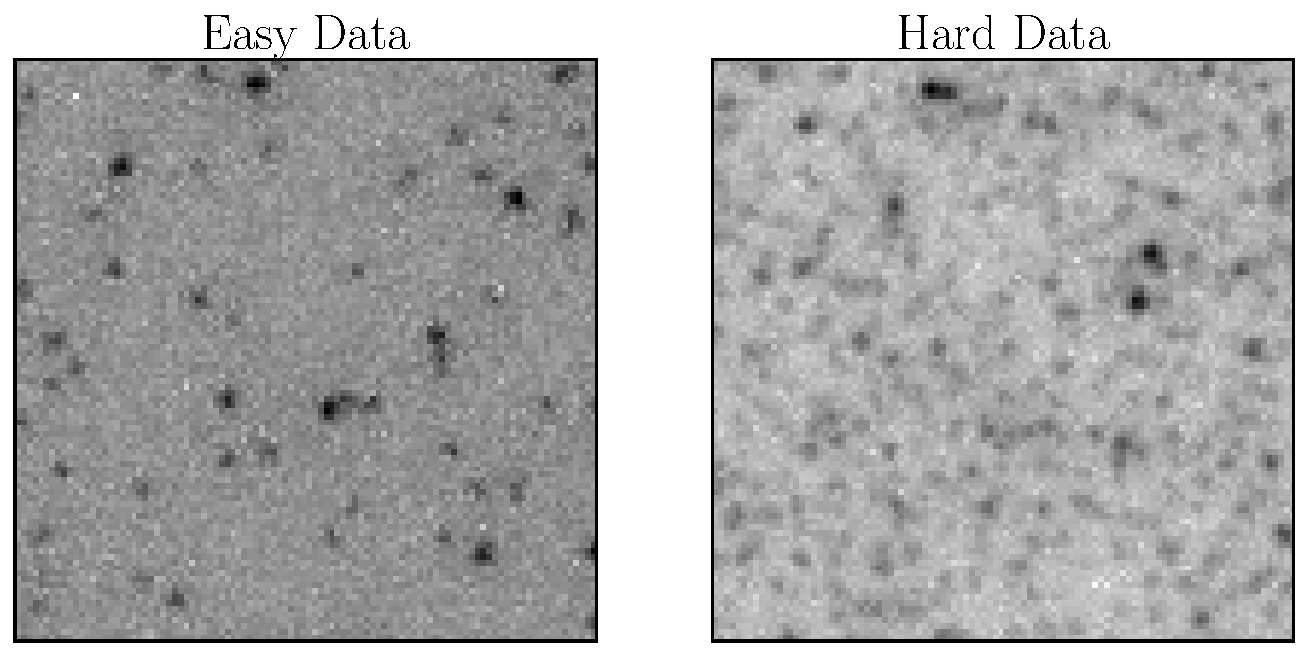
\includegraphics[scale=0.5]{Figures/data.pdf}
\caption{The two simulated datasets originally studied 
in \citet{starfield}. The ``easy'' image contains 100 stars and the
``hard'' image contains 1000. The goal is to infer the number $N$ of stars
in an image along with their positions and brightnesses.\label{fig:data}}
%\end{center}
\end{figure}

For the ``easy'' simulated data set containing 100 stars, the information
$H$ was approximately 500 nats, whereas for the ``hard'' dataset the information
was $\sim$2600 nats. In both cases, the upward part of the DNS run was
straightforward. However, in the ``hard'' case the diffusion phase of DNS
is very slow. Unfortunately, I am presently unaware of any Nested Sampling
method that only moves upwards in likelihood but is able to correct for the
use of imperfect MCMC. Variations of annealing or tempering such as
``annealed importance sampling'' and ``linked importance sampling'' \citep{ais, lis}
have both these properties, suggesting this may be possible with NS as well.





\subsection{Models with known oversimplifications}
Computing the posterior $p(\pars | \data)$ would yield overconfident results
since the assumed model is known to be wrong. However certain parameters still
``exist'' (such as the black hole mass) and we want our posterior inferences
to be realistic.

We have been using the following subjective procedure. Later we give two
interpretations of this procedure which may lead the way to less subjective
approaches.
Using DNS we explore the mixture of constrained priors.

where $X_i \approx e^{-i}$ by construction.

%%%%%%%%%%%%%%%%%%%%%%%%%%%%%%%%%%%%%%%%%%%%%%%%
%% BACKMATTER
%%%%%%%%%%%%%%%%%%%%%%%%%%%%%%%%%%%%%%%%%%%%%%%%

\begin{theacknowledgments}
It is a pleasure to thank David W. Hogg (NYU), Daniel Foreman-Mackey (NYU),
Fengji Hou (NYU), Anna Pancoast (UCSB), Benjamin Pope (Oxford), and
John Skilling (MaxEnt Data Consultants) for valuable discussions.
\end{theacknowledgments}

%%%%%%%%%%%%%%%%%%%%%%%%%%%%%%%%%%%%%%%%%%%%%%%%
%% The bibliography can be prepared using the BibTeX program or
%% manually.
%%
%% The code below assumes that BibTeX is used.  If the bibliography is
%% produced without BibTeX comment out the following lines and see the
%% aipguide.pdf for further information.
%%
%% For your convenience a manually coded example is appended
%% after the \end{document}
%%%%%%%%%%%%%%%%%%%%%%%%%%%%%%%%%%%%%%%%%%%%%%%%

%%%%%%%%%%%%%%%%%%%%%%%%%%%%%%%%%%%%%%%%%%%%%%%%
%% You may have to change the BibTeX style below, depending on your
%% setup or preferences.
%%
%%
%% For The AIP proceedings layouts use either
%%%%%%%%%%%%%%%%%%%%%%%%%%%%%%%%%%%%%%%%%%%%

\bibliographystyle{aipproc}   % if natbib is available
%\bibliographystyle{aipprocl} % if natbib is missing

%%%%%%%%%%%%%%%%%%%%%%%%%%%%%%%%%%%%%%%%%%%
%% You probably want to use your own bibtex database here
%%%%%%%%%%%%%%%%%%%%%%%%%%%%%%%%%%%%%%%%%%%
%\bibliography{sample}

%%%%%%%%%%%%%%%%%%%%%%%%%%%%%%%%%%%%%%%%%%%%
%%% Just a reminder that you may have to run bibtex
%%% All of it up to \end{document} can be removed
%%% if you don't like the warning.
%%%%%%%%%%%%%%%%%%%%%%%%%%%%%%%%%%%%%%%%%%%%
%\IfFileExists{\jobname.bbl}{}
% {\typeout{}
%  \typeout{******************************************}
%  \typeout{** Please run "bibtex \jobname" to optain}
%  \typeout{** the bibliography and then re-run LaTeX}
%  \typeout{** twice to fix the references!}
%  \typeout{******************************************}
%  \typeout{}
% }

\begin{thebibliography}{9}
\bibitem[Bertin and
Arnouts(1996)]{sextractor} Bertin, E., Arnouts, S.\ 1996.\ SExtractor: Software for source extraction.\ Astronomy and Astrophysics Supplement Series 117, 393-404.

\bibitem[Brewer et al.(2013)]{starfield} Brewer, B.~J., 
Foreman-Mackey, D., Hogg, D.~W.\ 2013.\ Probabilistic Catalogs for Crowded 
Stellar Fields.\ The Astronomical Journal 146, 7. 

\bibitem[Brewer et al.(2011)]{dnest}
Brewer, B.~J., P\'{a}rtay, L.~B., Cs\'{a}nyi, G.\ 2011.\
Diffusive Nested Sampling.\ Statistics and Computing, 2011, 21, 4, 649-656.

\bibitem[Caticha(2008)]{caticha} Caticha, A.\ 2008.\ Lectures 
on Probability, Entropy, and Statistical Physics.\ ArXiv e-prints 
arXiv:0808.0012. 

\bibitem[Cox(1946)]{cox} Cox, R.~T.\ 1946.\ Probability, 
Frequency and Reasonable Expectation.\ American Journal of Physics 14, 
1-13. 

\bibitem[Dolphin(2000)]{dolphot} Dolphin, A.~E.\ 2000, Publications of the
Astronomical Society of the Pacific, 112, 1383 

\bibitem[Feroz et al.(2009)]{multinest} Feroz, F., Hobson, M.~P., 
Bridges, M.\ 2009.\ MULTINEST: an efficient and robust Bayesian inference 
tool for cosmology and particle physics.\ Monthly Notices of the Royal 
Astronomical Society 398, 1601-1614. 

\bibitem[Feroz and Hobson(2014)]{2014MNRAS.437.3540F} Feroz, F., Hobson, 
M.~P.\ 2014.\ Bayesian analysis of radial velocity data of GJ667C with 
correlated noise: evidence for only two planets.\ Monthly Notices of the 
Royal Astronomical Society 437, 3540-3549. 

\bibitem[Hobson 
\& McLachlan(2003)]{2003MNRAS.338..765H} Hobson, M.~P., \& McLachlan, C.\ 2003, Monthly Notices of the Royal Astronomical Society, 338, 765 

\bibitem[Jaynes and Bretthorst(2003)]{jaynes} Jaynes, E.~T., 
Bretthorst, G.~L.\ 2003.\ Probability Theory.\ Probability Theory, by 
E.~T.~Jaynes and Edited by G.~Larry Bretthorst, pp.~758.~ISBN 
0521592712.~Cambridge, UK: Cambridge University Press, June 2003.\ . 

\bibitem[Lentati et al.(2014)]{2014MNRAS.437.3004L} Lentati, L., Alexander, 
P., Hobson, M.~P., Feroz, F., van Haasteren, R., Lee, K.~J., Shannon, 
R.~M.\ 2014.\ TEMPONEST: a Bayesian approach to pulsar timing analysis.\ 
Monthly Notices of the Royal Astronomical Society 437, 3004-3023. 

\bibitem[Marinari and Parisi(1992)]{simulated_tempering} Marinari, E., 
Parisi, G.\ 1992.\ Simulated tempering: a new Monte Carlo scheme.\ EPL 
(Europhysics Letters) 19, 451. 

\bibitem[Neal(1998)]{ais} Neal, R.~M.\ 1998.\ Annealed 
Importance Sampling.\ ArXiv Physics e-prints arXiv:physics/9803008. 

\bibitem[Neal(2005)]{lis} Neal, R.~M.\ 2005.\ Estimating 
Ratios of Normalizing Constants Using Linked Importance Sampling.\ ArXiv 
Mathematics e-prints arXiv:math/0511216. 

\bibitem[Skilling(1998)]{massinf} Skilling, J.\ 1998.\ Massive 
Inference and Maximum Entropy.\ Maximum Entropy and Bayesian Methods, 1. 

\bibitem[\protect\citeauthoryear{Skilling}{2006}]{skilling} Skilling, J., 2006, Nested Sampling for General Bayesian Computation, Bayesian Analysis 4, pp. 833-860.

\bibitem[Sutter et al.(2014)]{2014MNRAS.438..768S} Sutter, P.~M., Wandelt, 
B.~D., McEwen, J.~D., Bunn, E.~F., Karakci, A., Korotkov, A., Timbie, P., 
Tucker, G.~S., Zhang, L.\ 2014.\ Probabilistic image reconstruction for 
radio interferometers.\ Monthly Notices of the Royal Astronomical Society 
438, 768-778. 

\end{thebibliography}

\end{document}

%%%%%%%%%%%%%%%%%%%%%%%%%%%%%%%%%%%%%%%%%%%
%% The following lines show an example how to produce a bibliography
%% without the help of the BibTeX program. This could be used instead
%% of the above.
%%%%%%%%%%%%%%%%%%%%%%%%%%%%%%%%%%%%%%%%%%%



\endinput
%%
%% End of file `template-8s.tex'.
